\documentclass[pre,preprint,superscriptaddress]{revtex4-1} 

\usepackage{graphicx}
\usepackage{hyperref}
\usepackage{amsmath}
\usepackage{amsfonts} % needed for bold Greek, Fraktur, and blackboard bold
\usepackage{amssymb}
\usepackage[margin=1in]{geometry}
\usepackage{dcolumn}
\usepackage{multirow}
\usepackage{tikz}
\usetikzlibrary{calc,patterns,decorations.pathmorphing,decorations.markings}
\usepackage{hyperref}
\usepackage{float}
\usepackage{subfig}
\usepackage{todonotes}
\usepackage{subfiles}
\usepackage{morefloats}

% TODO: remove these lines, which expand the margins (useful for comments)
\textwidth  .72\paperwidth
\hoffset -1in
\oddsidemargin .14\paperwidth
\evensidemargin .14\paperwidth
\marginparwidth .11\paperwidth


% Draft macros
\usepackage[normalem]{ulem} % for strikethrough
%\usepackage[usenames,dvipsnames]{xcolor}
%\newcommand{\TODO}[1]{\marginpar{\raggedright\scriptsize\textbf{TODO:} #1} (\textbf{TODO})}
%\newcommand{\NOTEMARG}[1]{\marginpar{\raggedright\scriptsize\textbf{NOTE:} #1} (\textbf{NOTE})}
%\newcommand{\NOTE}[1]{\marginpar{\footnotesize\textbf{NOTE}} (\textbf{NOTE: #1})}
%\definecolor{purple}{rgb}{1,0,1}


\newcommand{\eq}[1]{eq.~\eqref{eq:#1}}
\newcommand{\eqs}[2]{eqs.~\eqref{eq:#1} and \eqref{eq:#2}}
\renewcommand{\sec}[1]{section~\ref{sec:#1}}
\newcommand{\secs}[2]{sections~\ref{sec:#1} and \ref{sec:#2}}
\newcommand{\subsec}[1]{section~\ref{subsec:#1}}
\newcommand{\subsubsec}[1]{section~\ref{subsubsec:#1}}
\newcommand{\app}[1]{appendix~\ref{app:#1}}
\newcommand{\fig}[1]{figure~\ref{fig:#1}}
\newcommand{\figs}[2]{figures~\ref{fig:#1} and \ref{fig:#2}}
\newcommand{\tab}[1]{table~\ref{tab:#1}}
\newcommand{\nn}{\nonumber}




\begin{document}

\title{Time dependent forcing in the Swift-- Hohenberg equation}
\author{Punit Gandhi}
 \email{punit\_gandhi@berkeley.edu}
\author{C\'edric Beaume}
\author{Edgar Knobloch}
 \email{knobloch@berkeley.edu}
\affiliation{Department of Physics, University of California, Berkeley CA 94720, USA}
\date{\today}

\begin{abstract}
This update includes figures that summarize all of the results obtained to date on the study of the Swift-Hohenberg Equation with a periodic forcing in time.  
\end{abstract}

\maketitle

\section{Introduction and definitions}
The equation we consider is: 
\begin{equation}
u_t= (r_0+ \rho \sin\omega t) u-\left(1+\partial_{x}^2\right)^2u+b u^2-u^3\label{eq:SHtd},
\end{equation}
which describes the dynamics of a real field $u$ over one spatial dimension in time.  We have rescaled the equation so that the critical wavenumber that defines the natural wavelength of the patterned state is unity.   The average value of the linear forcing term $r_0$, the amplitude of oscillation $\rho$, the frequency of oscillation $\omega$, and the strength quadratic nonlinearity $b$ are left as parameters of the system.

We track the location of the front of a localized solution using the first moment on half the domain.  
\begin{equation}
X_{cm}=\frac{1}{||u||} \int_{L/2}^{L/2}  |x| |u|^2 dx
\end{equation}
where 
\begin{equation}
||u||= \int_{L/2}^{L/2}  |u|^2 dx
\end{equation}


\section{bistability and localized solutions in SHE}
The caption of Fig.~\ref{fig:BurkeSHE}  taken from J. Burke et et al., describes the locations of bifurcations and relevant boundaries of the constant forcing version of this problem ( e.g. $\rho=0$) with $b=1.8$.  

\begin{figure}[!htb]\center
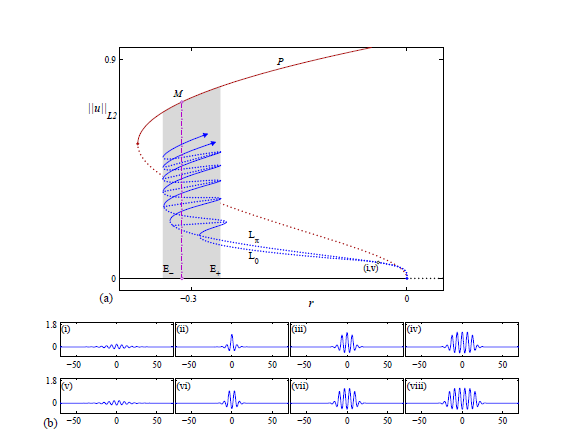
\includegraphics[width=120mm]{BurkeSHE.PNG}
\caption{\label{fig:BurkeSHE}This figure was taken from Burke\cite{} (a) Bifurcation diagram showing the snakes-and-ladders structure of localized states. Away from the origin the snaking branches $L_0$ and $L_-$ are contained within the snaking region (shaded) between$E_-$ and $E_+$, where $r(E_-)\approx -0.3390$ and $r(E_+)\approx -0.2593$.   Solid (dotted) lines indicate stable (unstable) states. In addition, the Maxwell point $M$, occurring at $r(M)\approx -0.3128$  is indicated with a vertical dash-dot line.  The saddle node bifurcation that creates the stable periodic state occurs at $r<r(SN_P)\approx -0.3744$, defining the left edge of the bistability region.  We will also find it useful to define the center of the snaking region $C$, which corresponds to  the forcing parameter $r(C)\approx -0.2992$. (b) Sample localized profiles $u(x): (i-iv)$ lie on $L_0$, near onset and at the 1st, 3rd, and 5th saddle-nodes from the bottom, respectively; (v-viii) lie on $L_-$, near onset and at the 1st, 3rd, and 5th saddle-nodes, respectively. Parameters: $b = 1.8$.} 
\end{figure}



\section{Numerical Methods}

All simulations in time used periodic boundary conditions and a domain of $80\pi$ (e.g. 40 characteristic wavelengths).  A 4th order exponential time differencing scheme\cite{cox2002} was used to step forward  in time while spectral methods on a grid of 1024 points were used for the spatial calculations.  Steady state solutions were computed by numerical continuation using AUTO~\cite{doedel1981auto}.   We will focus on SHE23 case with $b=1.8$, and study the dependence on the time-periodic forcing. We can vary the way the forcing oscillates ($r\rightarrow r_0+\rho \sin\omega t$) in 3 ways: (1) the amplitude of the oscillation, $\rho$ (2) the point about which the oscillation occurs, $r_0$ (3) the frequency with which the oscillation occurs, $\omega$.    unless otherwise noted,the simulations are initialized with a localized solution that is stable for the constant forcing ($\rho=0$) case with the given choice of $r_0$.  


\begin{figure}[!htb]
  \begin{center}
    \mbox{
      \subfloat[]{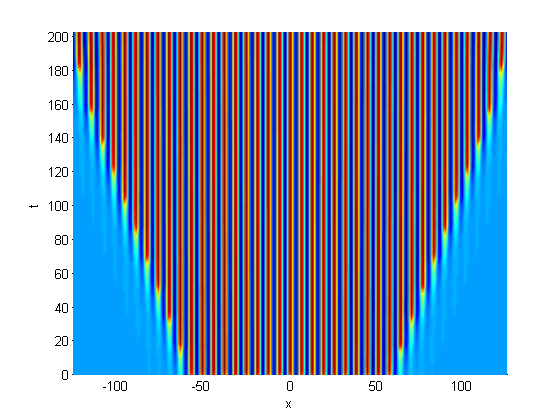
\includegraphics[width=60mm]{NucleationSolution.png}} \quad
      \subfloat[]{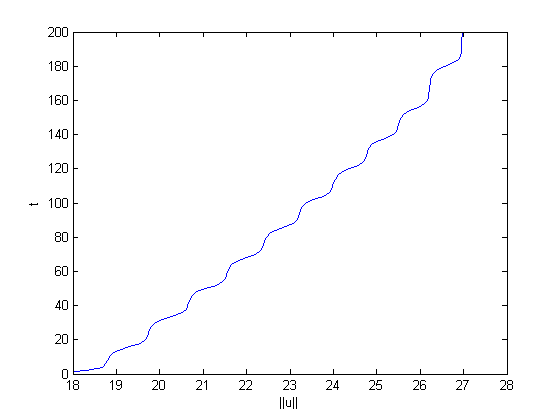
\includegraphics[width=60mm]{NucleationNorm.png} }
      }
    \caption{A simulation of the SHE with $N_{23}$, $b=1.8$ and $r=-0.20$ (e.g. $\delta\approx 0.06$) is initialized using a localized solution that is stable within the snaking region (e.g. at $r=-0.2944$). The solution growing in time (a) with red as high values and blue as low values.  The norm of the solution as it grows in time is shown in (b).  We note that the solution fills the domain with a period solution containing 39 periods on a domain of 40 characteristic wavelengths.}
    \label{fig:nucleation1}
  \end{center}
\end{figure}   


 \begin{figure}[!htb]
  \begin{center}
    \mbox{
      \subfloat[]{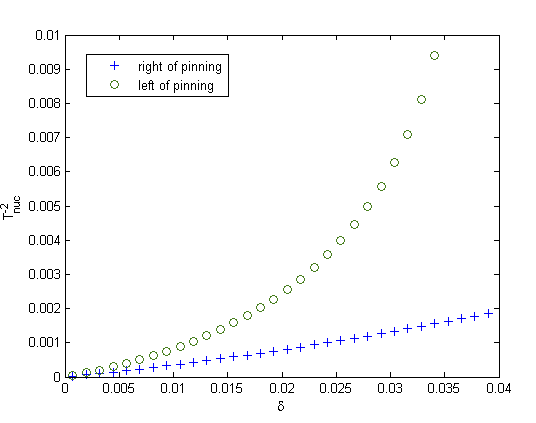
\includegraphics[width=60mm]{NucleationTime.png}} \quad
      \subfloat[]{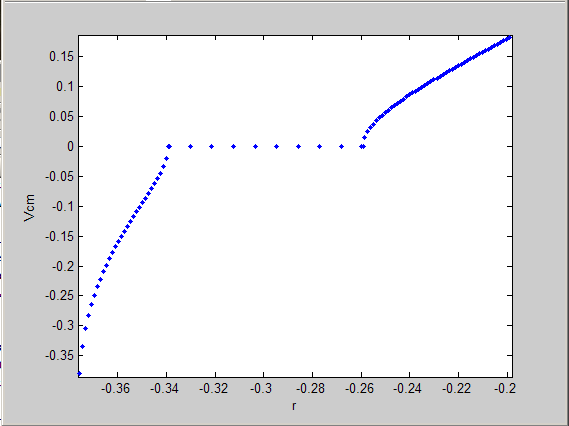
\includegraphics[width=60mm]{FrontSpeed.png} }
      }
    \caption{Simulation of the SHE with $N_{23}$ with $b=1.8$ show (a) $1/T_{nuc}^2$, where $T_{nuc}$ is the time between nucleation/decay events, as a function of distance from the edge of the pinning region  $\delta$, and (b) the front speed as a function of the forcing parameter. We note that the initial solution used in these simulations was on a saddle node bifurcation of snaking branch at the closest edge of the pinning region. }
    \label{fig:nucleation}
  \end{center}
\end{figure} 


\begin{figure}[!htb]\center
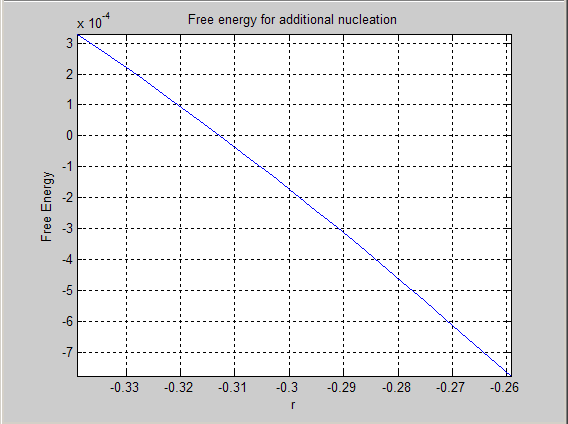
\includegraphics[width=80mm]{FEnucleation.png}
\caption{\label{fig:FEnuc} The difference in free energy between stable localized solutions that differ by 2 periods as a function of the forcing parameter $r$ in the SHE ($\rho=0$), with $b=1.8$.}
\end{figure}

\begin{figure}[!htb]\center
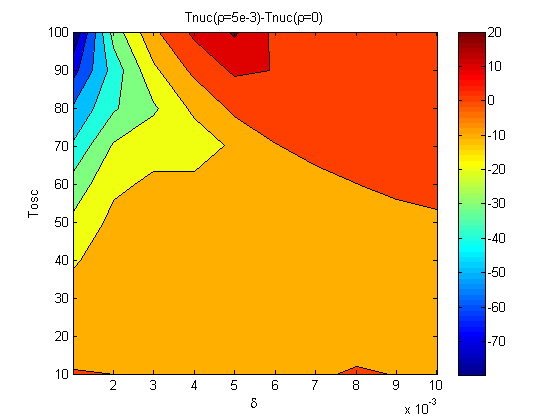
\includegraphics[width=80mm]{NucleationTimeOscDiff005.png}
\caption{difference in time between nucleation events for the $\rho=5\times10^{-3}$ case and the constant forcing case ($\rho=0$) as a function of distance from the right edge of the pinning region ($\delta$) and the period of oscillation.  The simulation was initialized with a localized solution that is stable at the right edge of the pinning region.}
    \label{fig:dTnuc}
\end{figure}

\begin{figure}[!htb]
\begin{center}
    \mbox{
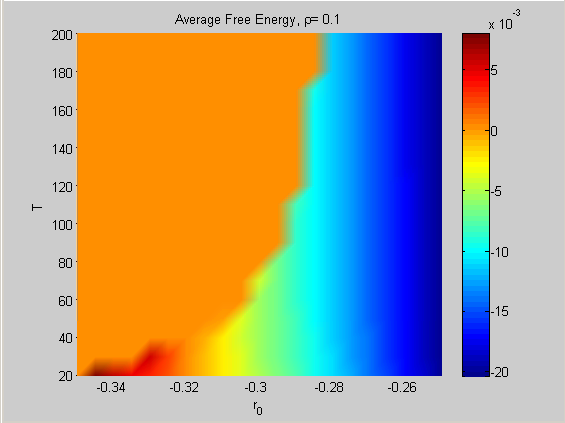
\includegraphics[width=50mm]{FEosc1.png}
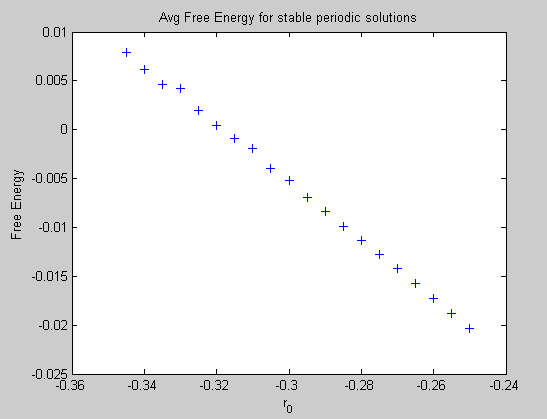
\includegraphics[width=50mm]{FEosc2.png}
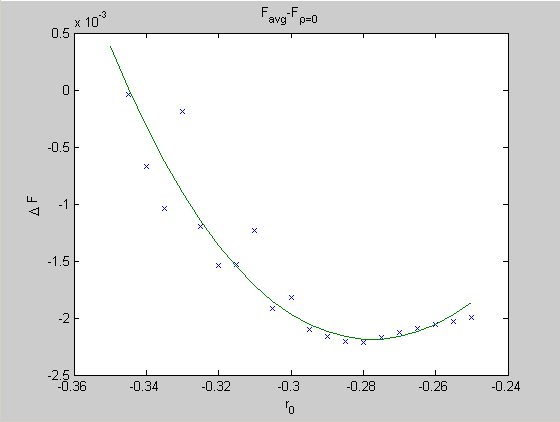
\includegraphics[width=50mm]{FEosc3.png}
}
\caption{(a)The average free energy along an oscillation for spatially periodic solutions that are als periodic in time under the time dependent forcing. The orange on the upper left corner indicates that the initial spatially periodic solution did not produce a stable oscillating solution in time. (b) The average free energy as a function of oscillation center for an oscillation period $T_{osc}=20$.  (c) The difference in free energy of the average of the oscillation and the constant forcing case.  The line represents the difference of a linear fit of the average free energy from the constant forcing case.   }
    \label{fig:FEosc}
\end{center}
\end{figure}


\begin{figure}[!htb]
  \begin{center}
    \mbox{
      \subfloat[]{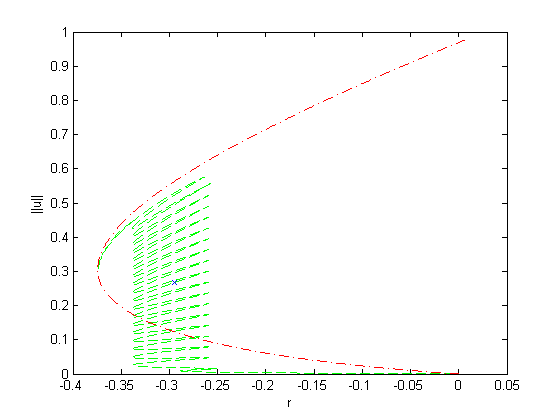
\includegraphics[width=60mm]{NormrBack.png}} \quad
      \subfloat[]{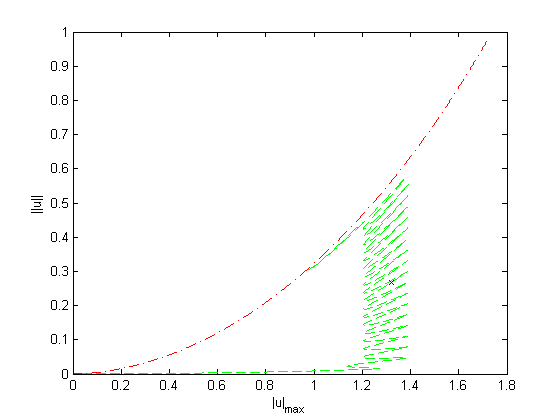
\includegraphics[width=60mm]{NormMaxBack.png} }
      }
    \caption{(a)A plot of the time-steady localized (green dash) and periodic (red dash-dot) solutions as a function of the forcing parameter in the problem with constant $r$ in time.  The blue x indicates the localized initial solution for the simulations with time-periodic forcing.  We note that future plots will zoom into the region near this x.  (b) This same data is plotted in terms of the max value vs L2 norm of the solutions in order to provide some reference for the trajectories of the time-dependent parameter case. }
    \label{fig:NormMaxBack}
  \end{center}
\end{figure} 

\begin{figure}[!htb]
  \begin{center}
    \mbox{
      	\subfloat[$\omega=4\pi$]{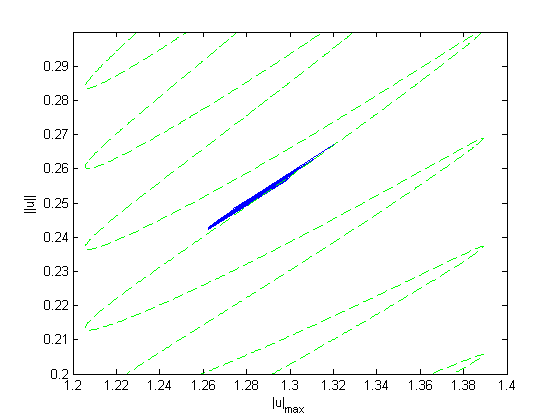
\includegraphics[width=40mm]{MinSnakingT05.png}} 
	\subfloat[$\omega=2\pi/5$]{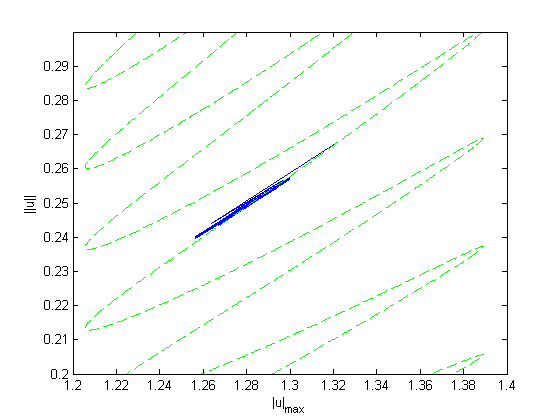
\includegraphics[width=40mm]{MinSnakingT5.png}} 
	\subfloat[$\omega=2\pi/50$]{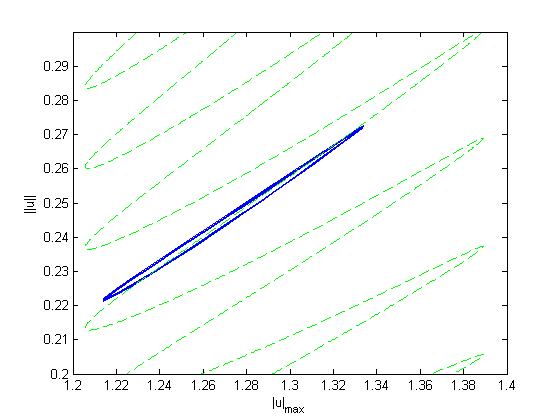
\includegraphics[width=40mm]{MinSnakingT50.png}}
      	\subfloat[$\omega=2\pi/500$]{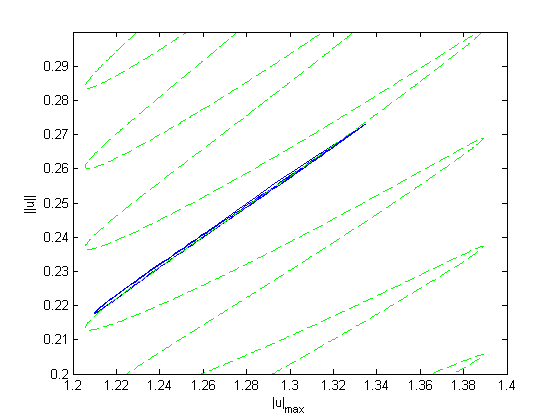
\includegraphics[width=40mm]{MinSnakingT500.png} }
      }
    \caption{Oscillations of the forcing parameter about the Maxwell point within the snaking region.  The forcing parameter as a function of time is given by $r\rightarrow-0.3128+ 0.025\sin\omega t$ for various values of $\omega$ (a)-(d).  Note that these figures are plotting the maximum value of the solution vs. its L2 norm just as in Fig.~\ref{fig:NormMaxBack} except that they are zoomed into a smaller region of the phase space slice centered around the initial condition (the blue x).  The time-independent snaking branch is also shown here for reference. }
    \label{fig:OscInSnake}
  \end{center}
\end{figure} 

\begin{figure}[!htb]
  \begin{center}
    \mbox{
      	\subfloat[$\omega=2\pi/50$]{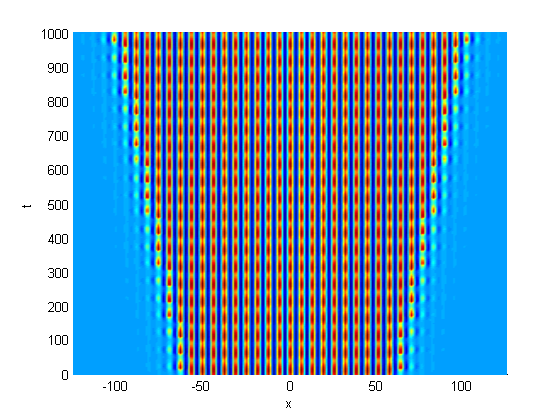
\includegraphics[width=50mm]{r0nD280drD10t050sol.png}} 
	\subfloat[$\omega=2\pi/100$]{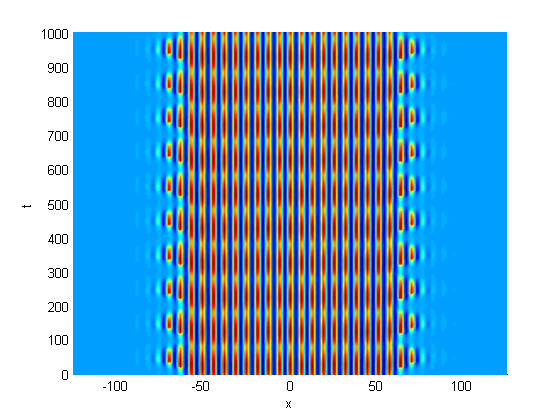
\includegraphics[width=50mm]{r0nD280drD10t100sol.png}} 
	\subfloat[$\omega=2\pi/200$]{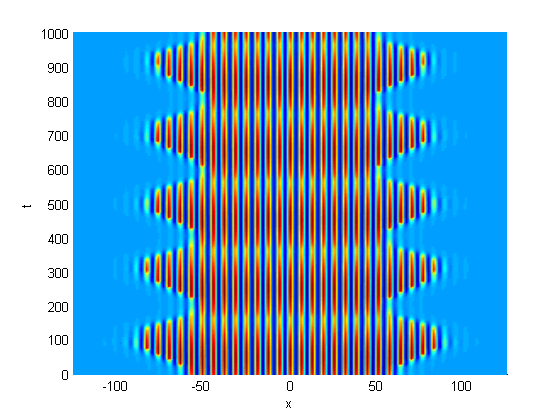
\includegraphics[width=50mm]{r0nD280drD10t200sol.png}} 
      } \mbox{
     	\subfloat[$\omega=2\pi/50$]{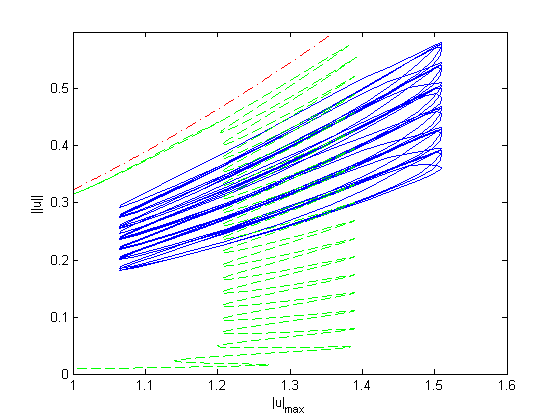
\includegraphics[width=50mm]{r0nD280drD10t050phase.png}} 
	\subfloat[$\omega=2\pi/100$]{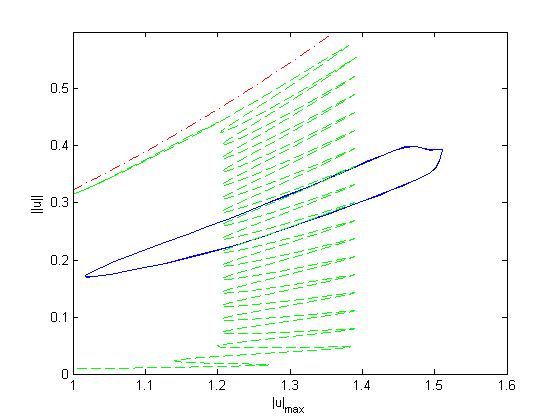
\includegraphics[width=50mm]{r0nD280drD10t100phase.png}} 
	\subfloat[$\omega=2\pi/200$]{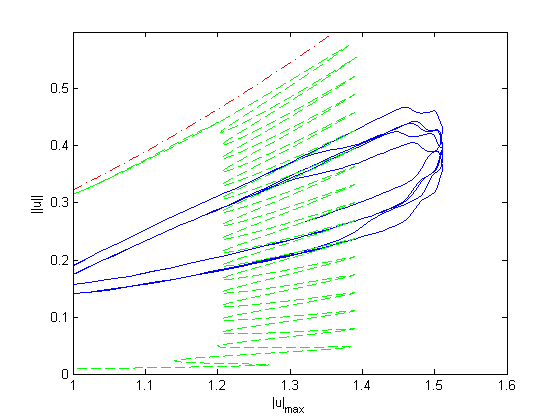
\includegraphics[width=50mm]{r0nD280drD10t200phase.png}}
}
    \caption{Oscillations of the forcing parameter in and out of the snaking region.  The forcing parameter as a function of time is given by $r\rightarrow -0.28+ 0.1\sin\omega t$ for various values of $\omega$. (a)-(c) show the solution as a function of time and (d)-(f) show the corresponding trajectories along the max value - L2 norm phase space slice (the time-independent snaking branch and periodic branches are also shown here for reference). }
    \label{fig:OscOutSnake}
  \end{center}
\end{figure}


\begin{figure}[!htb]\center
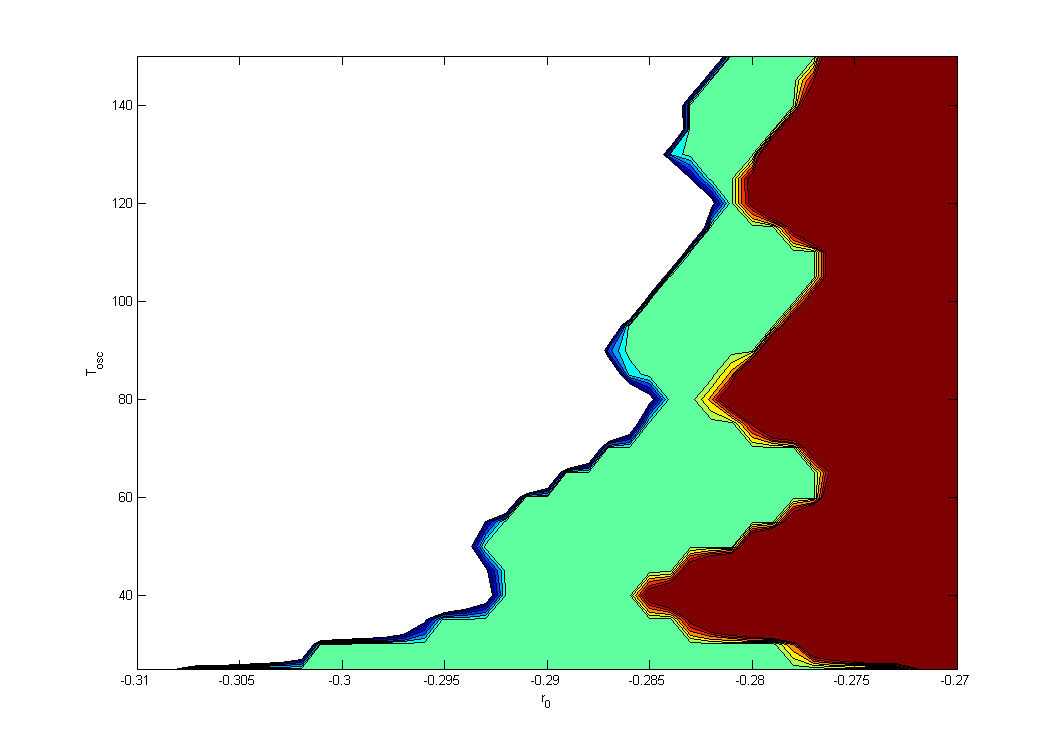
\includegraphics[width=120mm]{Vcm01.png}
\caption{The average speed at which the solution grows or decays as a function of oscillation period and oscillation center of the forcing parameter when $\rho=0.1$.  The solution had decayed by 6 or more periods over the course of the simulation (2000 units of time) in the white region, and has grown by six or more periods over the course of the simulation  in the red region.  The green region indicates where the solution has not grown or decayed on average.}
    \label{fig:Vcm01}
\end{figure}


\begin{figure}[!htb]\center
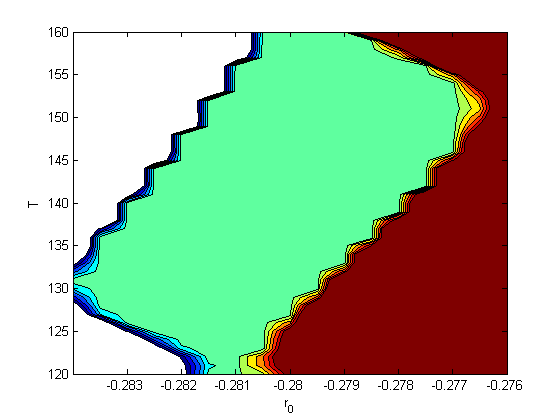
\includegraphics[width=120mm]{Vcm01zoom.png}
\caption{The average speed at which the solution grows or decays as a function of oscillation period and oscillation center of the forcing parameter.  The solution had decayed by 6 or more periods over the course of the simulation (2000 units of time) in the white region, and has grown by six or more periods over the course of the simulation  in the red region.  The green region indicates where the solution has not grown or decayed on average.}
    \label{fig:Vcm01zoom}
\end{figure}


\begin{figure}[!htb]
\begin{center}
    \mbox{
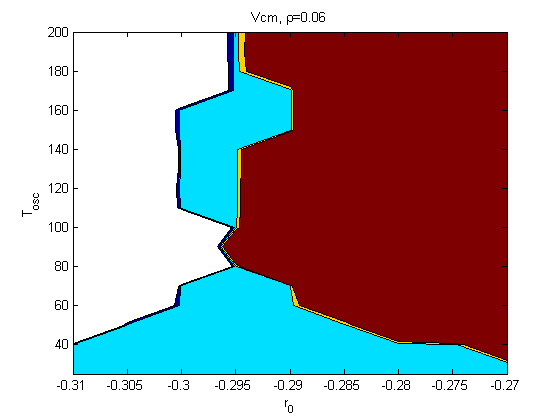
\includegraphics[width=50mm]{Vcm006error.png}
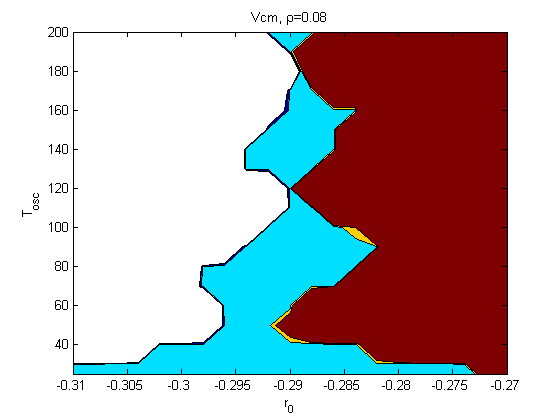
\includegraphics[width=50mm]{Vcm008.png}
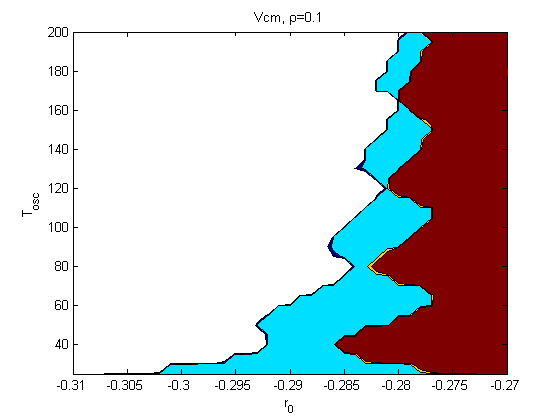
\includegraphics[width=50mm]{Vcm010.png}
}
\caption{The average speed at which the solution grows or decays as a function of oscillation period and oscillation center of the forcing parameter when (a)$\rho=0.06$, (b)$\rho=0.08$, (c)$\rho=0.1$.  The solution had decayed by 6 or more periods over the course of the simulation (2000 units of time) in the white region, and has grown by six or more periods over the course of the simulation  in the red region.  The green region indicates where the solution has not grown or decayed on average.}
    \label{fig:VcmCompare}
\end{center}
\end{figure}



\begin{figure}[!htb]
\begin{center}
    \mbox{
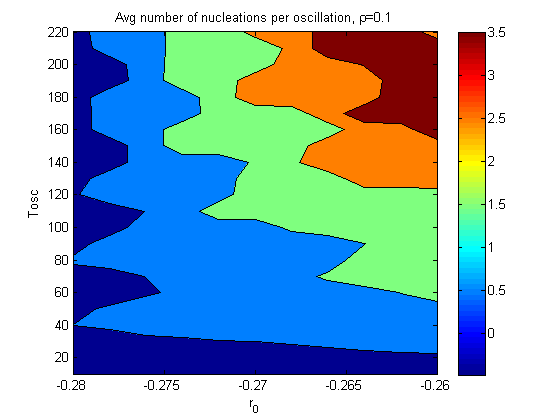
\includegraphics[width=50mm]{NucPerOsc.png}
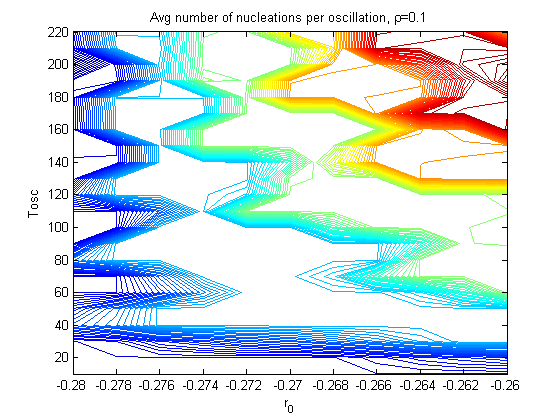
\includegraphics[width=50mm]{NucPerOscCont.png}
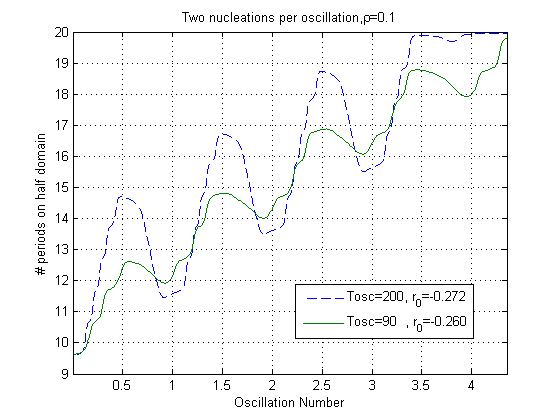
\includegraphics[width=50mm]{NucPerOsc2time.png}
}
\caption{Nucleations per oscillation. (a)The number of nucleations per oscillation ($V_{cm} T_{osc}/\pi$)  are indicated in these graphs with varying $T_{\text{osc}}$ and $r_0$, but fixed oscillation amplitude of $\rho=0.1$.  The dark blue indicates the region that is stable on average, the solution grows by one period on each side after each oscillation in the light blue, two on each side in the green, and so on.  We note the bit of orange in the upper right corner that needs further investigation.  (b) A graph of the same data is shown with 100 evenly spaced contour lines in order to emphasize that the boundaries between the regions are relatively sharp.  (c) The location of the front as a function of time are shown for two different points within the one nucleation per oscillation region. }
\label{fig:holes}
\end{center}
\end{figure}



\begin{figure}[!htb]\center
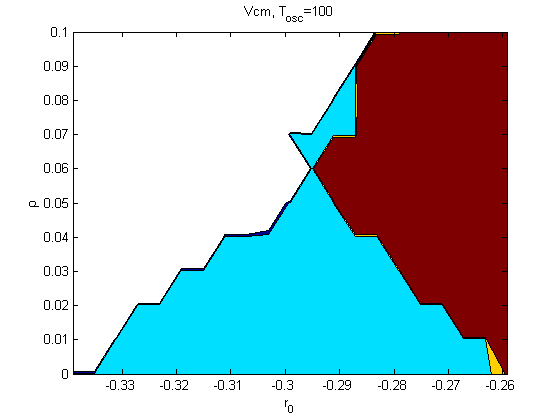
\includegraphics[width=120mm]{Vcm100.png}
\caption{The average speed at which the solution grows or decays as a function of oscillation amplitude and oscillation center of the forcing parameter when $T_{osc}=100$.  The solution had decayed by six or more periods over the course of the simulation (2000 units of time) in the white region, and has grown by six or more periods over the course of the simulation  in the red region.  The green region indicates where the solution has not grown or decayed on average.}
    \label{fig:Vcm100}
\end{figure}

\begin{figure}[!htb]
\begin{center}
    \mbox{
      \subfloat[]{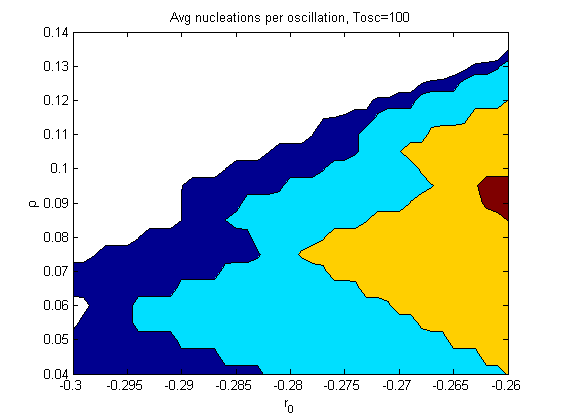
\includegraphics[width=60mm]{NucPerOscT100.png}} \quad
      \subfloat[]{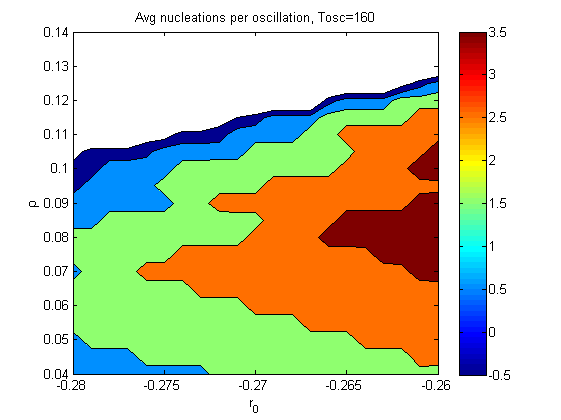
\includegraphics[width=60mm]{NucPerOscT160} }
      }
    \caption{Instead of plotting the speed of the front (e.g. Vcm), the number of nucleations per oscillation are indicated in these graphs with varying $\rho$ and $r_0$, but fixed oscillation period at (a)100 and (b) 160.  The dark blue regions in both graphs indicate the regions of localized solutions that do not grow on average.  The colored regions increase in nucleations per oscillations successively.  The color directly to the right of dark blue indicates one nucleation (of a period on each side of the solution) per oscillation, the next one over to the right indicates two nucleations per oscillation, and so on.  The solution decayed by one or more period  }
    \label{fig:NucPerOscT}
  \end{center}
\end{figure} 




 \begin{figure}[!htb]
  \begin{center}
    \mbox{
      	\subfloat[]{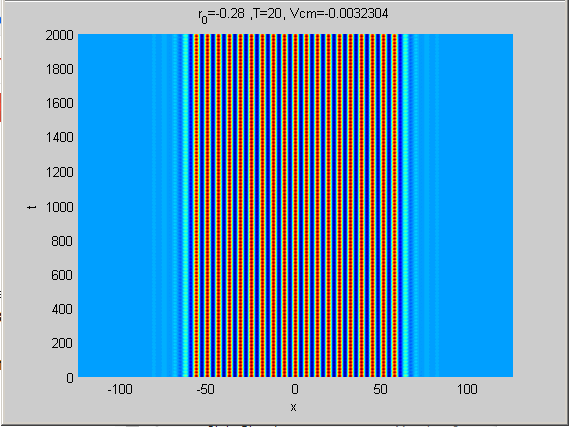
\includegraphics[width=60mm]{r0nD28drD10t020sol.png}}\quad 
      	\subfloat[]{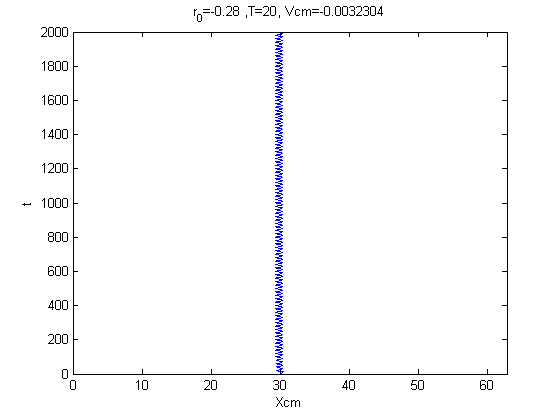
\includegraphics[width=60mm]{r0nD28drD10t020Xcm.png}} 
      } \mbox{
      	\subfloat[]{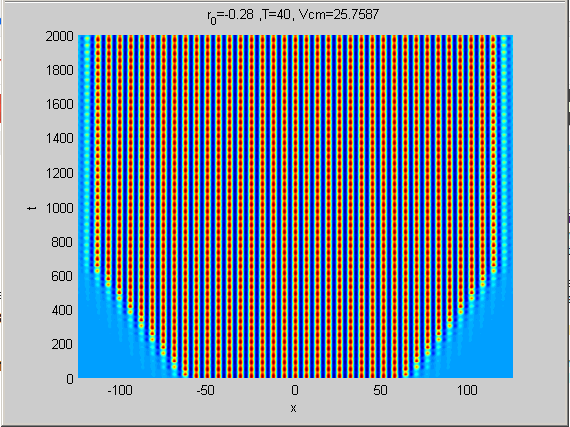
\includegraphics[width=60mm]{r0nD28drD10t040sol.png} }\quad 
	\subfloat[]{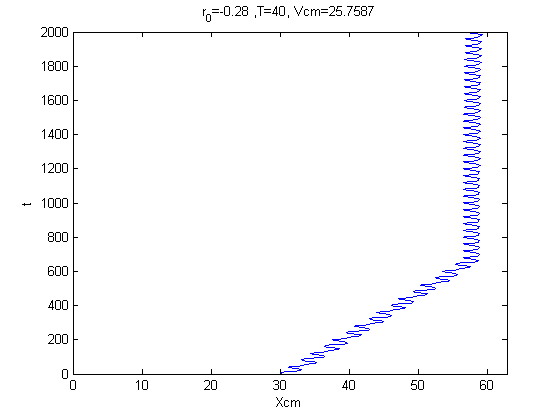
\includegraphics[width=60mm]{r0nD28drD10t040Xcm.png} }
      }
    \caption{Solutions along with Xcm are shown as  function of time for a series of oscillation periods at a fixed value of $r_0=-0.28$.  We see that the solution oscillates between growing and stable for this region, as expected given Fig.~\ref{fig:Vcm01}.  The value of $V_{cm}$ is given in number of periods nucleated or decayed over the course of the simulation (2000 units of time), assuming no boundary.}
    \label{fig:r28slice1}
  \end{center}
\end{figure} 

 \begin{figure}[!htb]
  \begin{center}
        \mbox{
	\subfloat[]{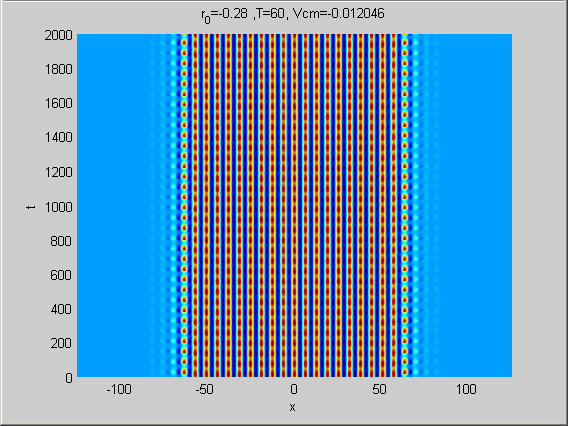
\includegraphics[width=60mm]{r0nD28drD10t060sol.png} }\quad 
	\subfloat[]{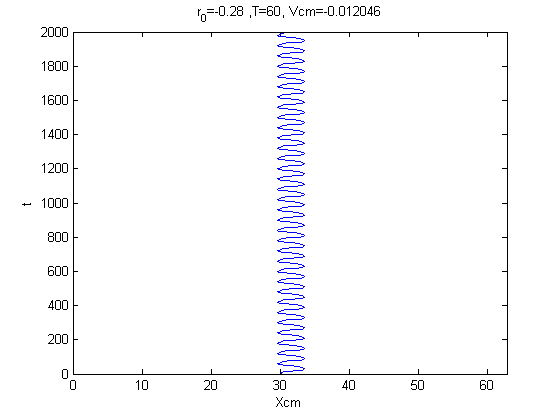
\includegraphics[width=60mm]{r0nD28drD10t060Xcm.png} }
      } \mbox{
	\subfloat[]{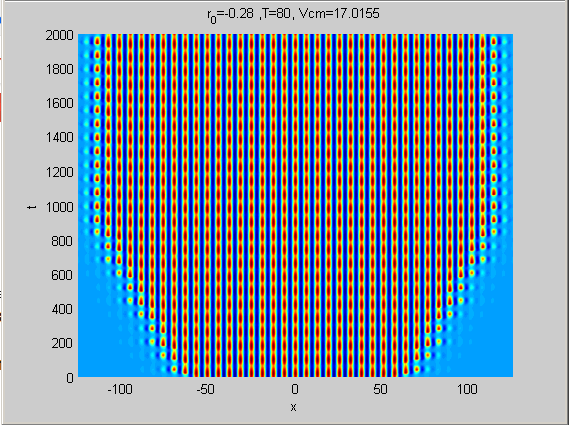
\includegraphics[width=60mm]{r0nD28drD10t080sol.png} }\quad
	\subfloat[]{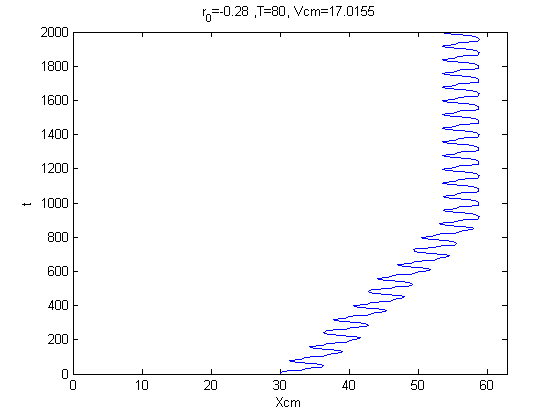
\includegraphics[width=60mm]{r0nD28drD10t080Xcm.png} }
      }
    \caption{Solutions along with Xcm are shown as  function of time for a series of oscillation periods at a fixed value of $r_0=-0.28$.  We see that the solution oscillates between growing and stable for this region, as expected given Fig.~\ref{fig:Vcm01}.  The value of $V_{cm}$ is given in number of periods nucleated or decayed over the course of the simulation (2000 units of time), assuming no boundary.}
    \label{fig:r28slice2}
  \end{center}
\end{figure} 

  \begin{figure}[!htb]
  \begin{center}
    \mbox{	
	\subfloat[]{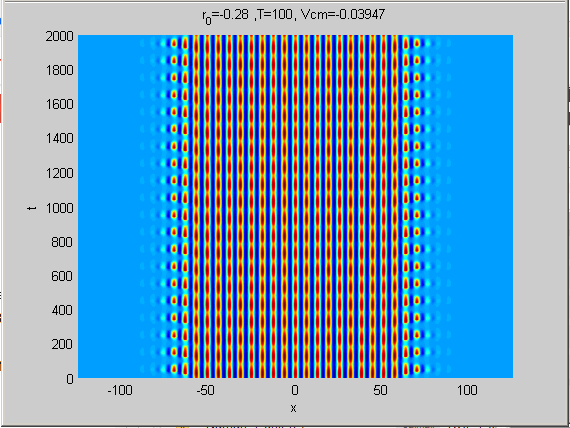
\includegraphics[width=60mm]{r0nD28drD10t100sol.png} }\quad 
	\subfloat[]{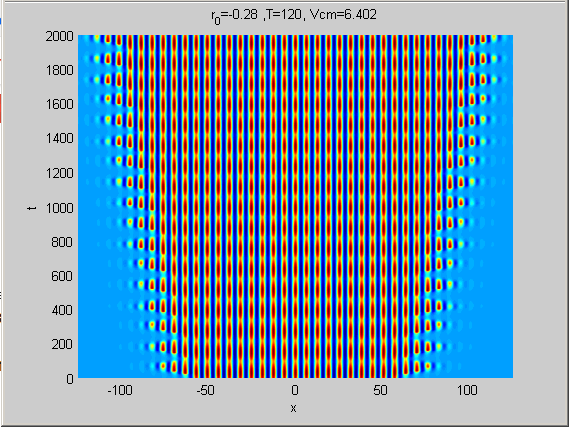
\includegraphics[width=60mm]{r0nD28drD10t120sol.png} } 
      } \mbox{
	\subfloat[]{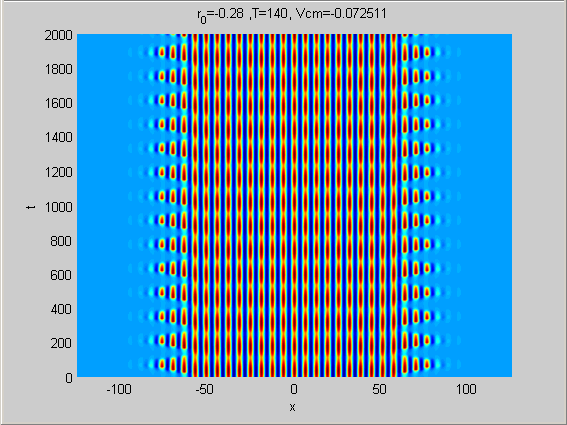
\includegraphics[width=60mm]{r0nD28drD10t140sol.png} }\quad 
	\subfloat[]{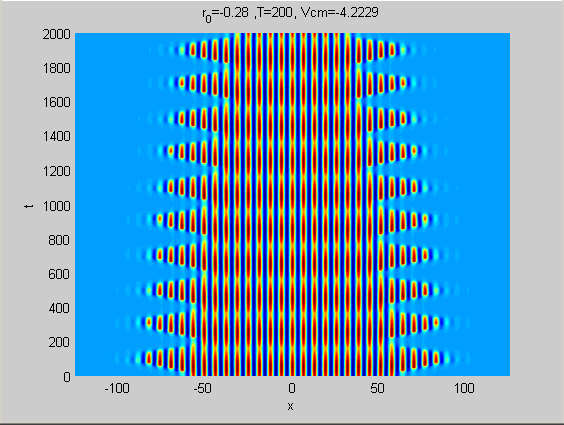
\includegraphics[width=60mm]{r0nD28drD10t200sol.png} } 
      }
    \caption{The pattern of oscillating between stable and growing solution continues up to about $T_{osc}=140$ and then, after a longer region of stability, the solutions oscillate between stable and decaying. The value of $V_{cm}$ is given in number of periods nucleated or decayed over the course of the simulation (2000 units of time), assuming no boundary.}
    \label{fig:r28slice3}
  \end{center}
\end{figure} 

\begin{figure}[!htb]
\begin{center}
    \mbox{
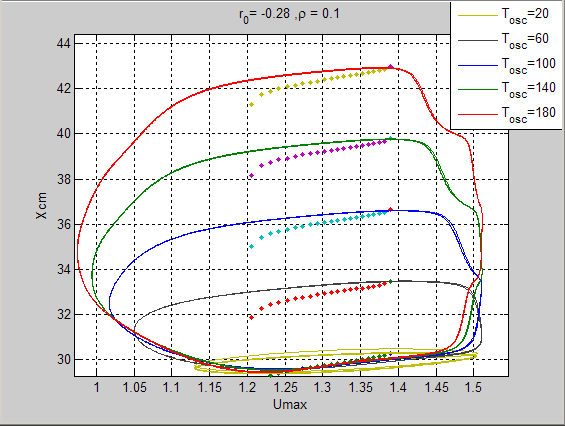
\includegraphics[width=50mm]{XumaxStable.png}
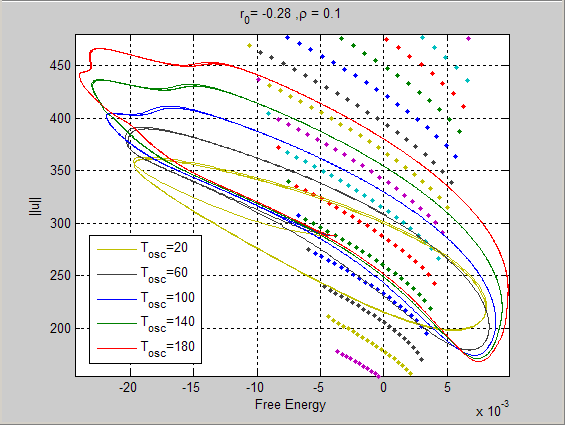
\includegraphics[width=50mm]{FEnormStable.png}
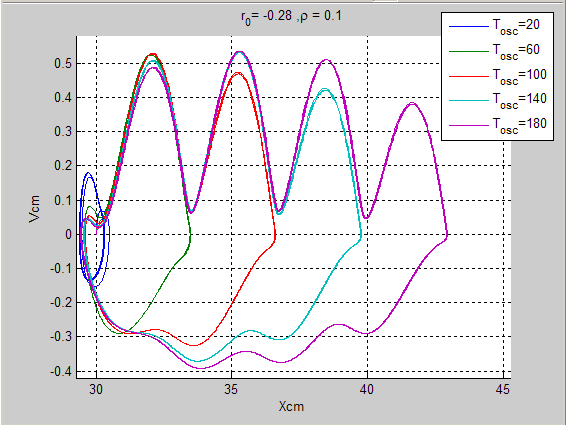
\includegraphics[width=50mm]{FrontPhase.png}
}
\caption{Various phase space slices of solutions along $r_0=-.28$ with $\rho=-0.1$ that are periodic in time.  (a)The maximum height of the solution vs the position of the front.  the motivation here was to graph the length and heigth of the solution to give some sense of its size.  (b) The free energy of the solution vs the L2 norm. (c) the phase space of the front, the postion of the front vs its speed.  }
    \label{fig:PhaseSlice}
\end{center}
\end{figure}



\begin{figure}[!htb]\center
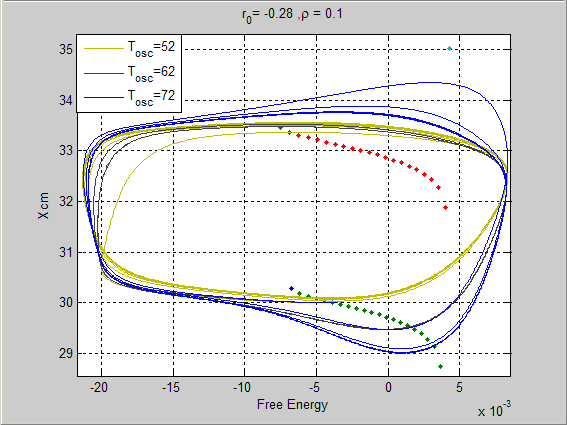
\includegraphics[width=80mm]{XcmFEstablerange.png}
\caption{Trajectories in phase space of  an orbit at the edges and center of the stable region in parameter space.}
    \label{fig:PhaseSlice2}
\end{figure}

\begin{figure}[!htb]
\begin{center}
    \mbox{
      \subfloat[]{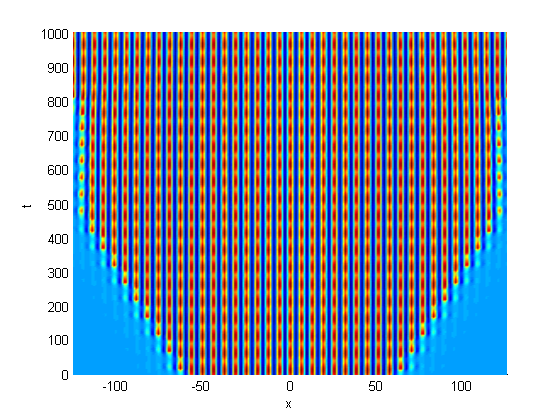
\includegraphics[width=60mm]{r0nD270drD10t050sol.png}} \quad
      \subfloat[]{\includegraphics[width=60mm]{r0nD270drD10t050phase.png} }
      }
    \caption{Oscillations of the forcing parameter in and out of the snaking region.  The forcing parameter as a function of time is given by $r\rightarrow -0.27+ 0.1\sin2\pi t/T_{osc}$.  The solution (a) grows in time, eventually filling the domain and the corresponding trajectory along the max value - L2 norm phase space slice (b) shows the path taken as it passes in and out of the snaking region. }
    \label{fig:FillDomain}
  \end{center}
\end{figure} 


\begin{figure}[!htb]
\begin{center}
    \mbox{
\includegraphics[width=50mm]{HoleQuasiStableT100rD275.png}
\includegraphics[width=50mm]{HoleStableT80rD275.png}
\includegraphics[width=50mm]{HoleStableT80rD275sol.png}
}
\caption{Stable and quasi-stable "hole" states in long-time simulations initialized with $\rho=0.1$, $r_0=-0.275$.  (a)$T_{\text{osc}}=100$ produces a quasistable hole stat that eventually grows into a periodic solution with 40 periods on the domain.    (b) $T_{\text{osc}}=80$ produces a stable defect state that has been presists for simulations all the way to T=20,000.  The norm of the difference of the solution at the same phase of each oscillation decays exponentially, indicated the solution is infact stable.  (c) The stable solution is shown as afunction of $x$ at $T=5000$  }
    \label{fig:holes}
\end{center}
\end{figure}

\begin{figure}[!htb]\center
\includegraphics[width=80mm]{StableDefectV0.png}
\caption{Region of stability of hole states in parameter space.  A hole state is initialized with $\rho=0.1$ for different values of $r_0$ and $T_{\text{osc}}$, and the ratio of the value of the field at the center to that at the edge at T=20,000 is plotted here.  The blue region corresponds to solutions that had a hole at the center of the domain persist for the entire simulation.  The red regions correspond to where a peak has formed at the center, indicated that the simulation has settled on a periodic solution with 40 periods.  The dark blue region corresponds to small negative troughs at the center of the domain, indicated that a periodic solution of 39 periods has been reached.  The white corresponds to regions where a localized solution remains stable on average.}
    \label{fig:holestability}
\end{figure}




\bibliography{TimeForcingSHE_bibliography}

\end{document}
